\documentclass[12pt,a4paper,titlepage]{article}
\usepackage[utf8]{inputenc}
\usepackage[french]{babel}
\usepackage[T1]{fontenc}
\usepackage{amsmath}
\usepackage{amsthm}
\usepackage{amsfonts}
\usepackage{amssymb}
\usepackage{graphicx}
\usepackage{url}
\usepackage{color}
\usepackage{listings}
\usepackage{mathrsfs}

\title{OS13 : Test d'estimation et loi extrême des lois de Cauchy et géométrique}
\author{\textsc{Adrien WARTELLE} \\ \textsc{TRAN Quoc Nhat Han}}
\date{\today}
\lstset{
language=R,
basicstyle=\scriptsize\ttfamily,
commentstyle=\ttfamily\color{green},
numbers=left,
numberstyle=\ttfamily\color{black}\footnotesize,
stepnumber=1,
numbersep=5pt,
backgroundcolor=\color{white},
showspaces=false,
showstringspaces=false,
showtabs=false,
frame=single,
tabsize=2,
captionpos=b,
breaklines=true,
breakatwhitespace=false,
keywordstyle=\color{blue},
stringstyle=\color{magenta},
literate=
  {á}{{\'a}}1 {é}{{\'e}}1 {í}{{\'i}}1 {ó}{{\'o}}1 {ú}{{\'u}}1
  {Á}{{\'A}}1 {É}{{\'E}}1 {Í}{{\'I}}1 {Ó}{{\'O}}1 {Ú}{{\'U}}1
  {à}{{\`a}}1 {è}{{\`e}}1 {ì}{{\`i}}1 {ò}{{\`o}}1 {ù}{{\`u}}1
  {À}{{\`A}}1 {È}{{\'E}}1 {Ì}{{\`I}}1 {Ò}{{\`O}}1 {Ù}{{\`U}}1
  {ä}{{\"a}}1 {ë}{{\"e}}1 {ï}{{\"i}}1 {ö}{{\"o}}1 {ü}{{\"u}}1
  {Ä}{{\"A}}1 {Ë}{{\"E}}1 {Ï}{{\"I}}1 {Ö}{{\"O}}1 {Ü}{{\"U}}1
  {â}{{\^a}}1 {ê}{{\^e}}1 {î}{{\^i}}1 {ô}{{\^o}}1 {û}{{\^u}}1
  {Â}{{\^A}}1 {Ê}{{\^E}}1 {Î}{{\^I}}1 {Ô}{{\^O}}1 {Û}{{\^U}}1
  {œ}{{\oe}}1 {Œ}{{\OE}}1 {æ}{{\ae}}1 {Æ}{{\AE}}1 {ß}{{\ss}}1
  {ű}{{\H{u}}}1 {Ű}{{\H{U}}}1 {ő}{{\H{o}}}1 {Ő}{{\H{O}}}1
  {ç}{{\c c}}1 {Ç}{{\c C}}1 {ø}{{\o}}1 {å}{{\r a}}1 {Å}{{\r A}}1
  {€}{{\EUR}}1 {£}{{\pounds}}1
}
\numberwithin{equation}{section}

\definecolor{mygreen}{RGB}{28,172,0} % color values Red, Green, Blue
\definecolor{mylilas}{RGB}{170,55,241}
\lstset{language=Matlab,%
    %basicstyle=\color{red},
    breaklines=true,%
    morekeywords={matlab2tikz},
    keywordstyle=\color{blue},%
    morekeywords=[2]{1}, keywordstyle=[2]{\color{black}},
    identifierstyle=\color{black},%
    stringstyle=\color{mylilas},
    commentstyle=\color{mygreen},%
    showstringspaces=false,%without this there will be a symbol in the places where there is a space
    numbers=left,%
    numberstyle={\tiny \color{black}},% size of the numbers
    numbersep=9pt, % this defines how far the numbers are from the text
    emph=[1]{for,end,break},emphstyle=[1]\color{red}, %some words to emphasise
    %emph=[2]{word1,word2}, emphstyle=[2]{style},    
}

\begin{document}
\maketitle 
\renewcommand{\contentsname}{Sommaire}
\tableofcontents

\clearpage

\begin{abstract}
Ce rapport est à montrer l'application de certaines tests statistiques pour la loi géométrique et la loi de Cauchy.
\end{abstract}

\section{Loi de Cauchy}
\subsection{Rappel}
Soit $f_X$ la fonction de densité de Cauchy de deux paramètres $x_0$ et $a$ ($a>0$), définie par:
\begin{equation}
\label{dCauchy}
{f_X}\left( x \right) = \frac{1}{{\pi a\left( {1 + {{\left( {\frac{{x - {x_0}}}{a}} \right)}^2}} \right)}} = \frac{1}{\pi }\frac{a}{{{{\left( {x - {x_0}} \right)}^2} + a}}
\end{equation}

\begin{figure}[h]
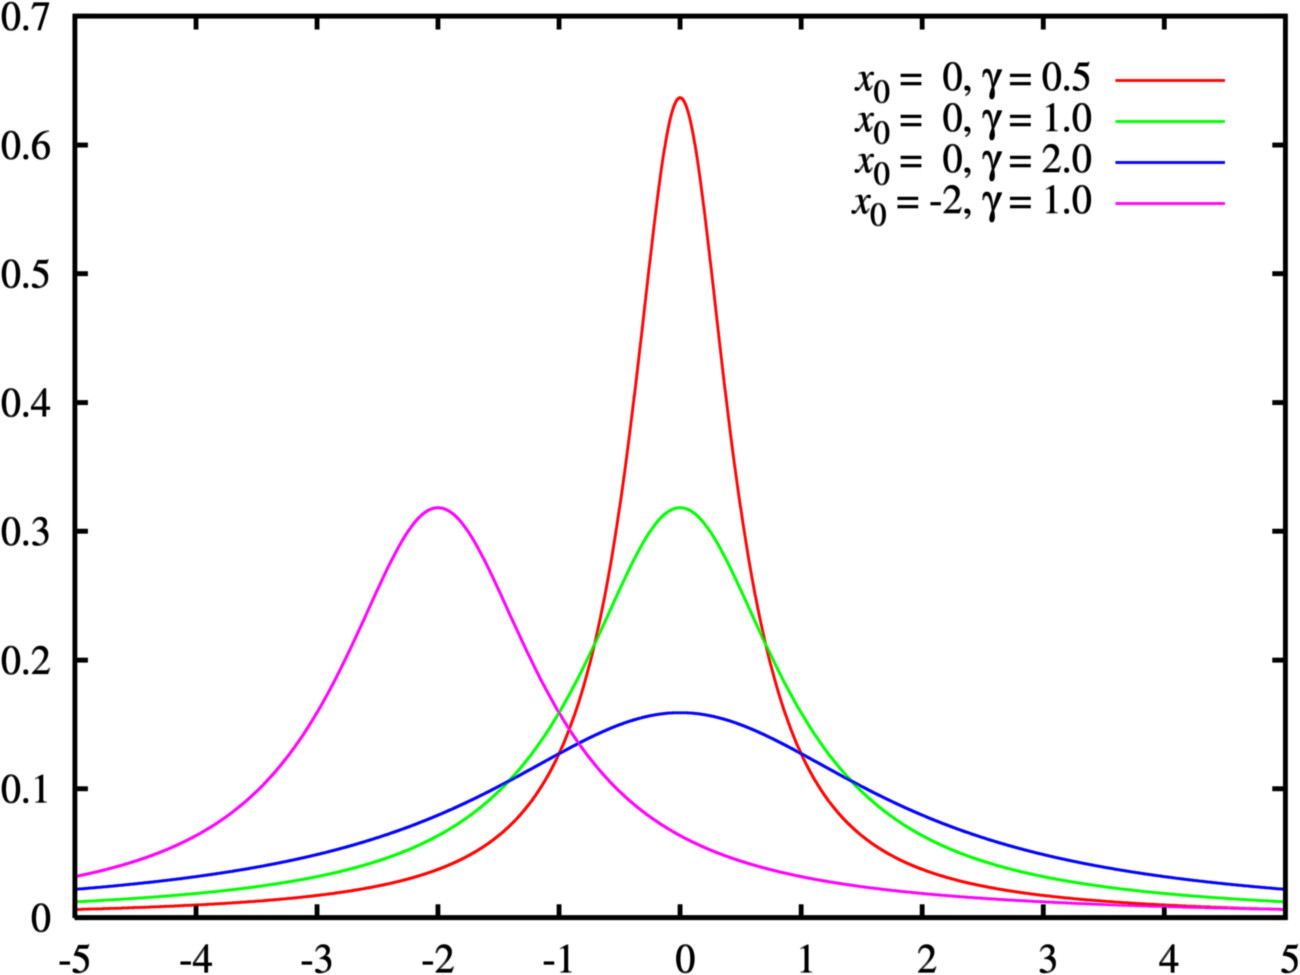
\includegraphics[width=\linewidth]{images/Cauchy_distribution_theoretic.png}
\caption{Distribution théorique de la loi Cauchy. Source : \cite{WikiLoiCauchy}}
\end{figure}

$a$ est dite l'échelle de la fonction, et $x_0$ est son médian.

La loi de Cauchy n'admet ni espérance ni écart type.

La fonction de répartition:
\begin{equation}
\label{rCauchy}
{F_X}\left( x \right) = \frac{1}{\pi }\arctan \left( {\frac{{x - {x_0}}}{a}} \right) + \frac{1}{2}
\end{equation}

\subsection{Estimer les paramètres inconnus}

\subsubsection*{Calcul théorique}

Soient $n$ réalisations $x_1, x_2, ..., x_n$. Assumons que ces données suivent la loi de Cauchy \eqref{dCauchy}.

Nous allons utiliser la méthode de maximum de rapport de vraisemblance.

En l'absence d'information de la distribution, nous assumons que ces mesures sont indépendants. Posons une variable aléatoire $X_i$ correspondante à chaque réalisation $x_i$ pour $i=\overline{1, n}$.

On écrit la loi conjointe de ces $n$ variables:

\begin{align*}
L (X) = L\left( {{X_1},{X_2},...,{X_n}} \right) & = \prod\limits_{i = 1}^n {{f_X}\left( {{X_i}} \right)} \\
& = \prod\limits_{i = 1}^n {\frac{1}{\pi }\frac{a}{{{{\left( {{x_i} - {x_0}} \right)}^2} + a}}} \\
& = {\pi ^{ - n}}\prod\limits_{i = 1}^n {\frac{a}{{{{\left( {{x_i} - {x_0}} \right)}^2} + a}}}
\end{align*}

On cherche l'optimum maximale.

\begin{align*}
\frac{{\partial L}}{{\partial {x_0}}}\left( X \right) & = {\pi ^{ - n}}\sum\limits_{j = 1}^n {\left( { - \frac{{a\left( {2{x_j} - 2{x_0}} \right)}}{{{{\left[ {{{\left( {{x_0} - {x_j}} \right)}^2} + a} \right]}^2}}}\prod\limits_{i = 1;i \ne j}^n {\frac{a}{{{{\left( {{x_i} - {x_0}} \right)}^2} + a}}} } \right)}\\
&  = {\pi ^{ - n}}\left( {\prod\limits_{i = 1}^n {\frac{a}{{{{\left( {{x_i} - {x_0}} \right)}^2} + a}}} } \right)\left( { - \sum\limits_{j = 1}^n {\frac{{2{x_0} - 2{x_j}}}{{{{\left( {{x_0} - {x_j}} \right)}^2} + a}}} } \right) \\
\frac{{\partial L}}{{\partial {x_0}}}\left( X \right) & = 0 \Leftrightarrow \sum\limits_{j = 1}^n {\frac{{{x_0} - {x_j}}}{{{{\left( {{x_0} - {x_j}} \right)}^2} + a}}}  = 0 \text{ : insolvable par la main}
\end{align*}

\begin{align*}
\frac{{\partial L}}{{\partial a}}\left( X \right) & = {\pi ^{ - n}}\sum\limits_{j = 1}^n {\left( {\frac{{{{\left( {{x_j} - {x_0}} \right)}^2} + a - a}}{{{{\left( {{x_j} - {x_0}} \right)}^2} + a}}\prod\limits_{i = 1;i \ne j}^n {\frac{a}{{{{\left( {{x_i} - {x_0}} \right)}^2} + a}}} } \right)}\\
&  = {\pi ^{ - n}}{a^{n - 1}}\frac{{\sum\limits_{j = 1}^n {{{\left( {{x_0} - {x_j}} \right)}^2}} }}{{\prod\limits_{i = 1}^n {\left( {{{\left( {{x_i} - {x_0}} \right)}^2} + a} \right)} }} > 0 \forall a > 0
\end{align*}

\subsubsection*{Résolution par R}

On génère une échantillon avec $a$ et $x_0$ au choix. Puis, utiliser la fonction $mle$ (Maximum Likelihood Estimator) de librairie \emph{stats4} avec 2 valeurs initiales $\hat{a}$ et $\hat{x_0}$ pour estimer $a$ et $x_0$.

Nous essayons d'estimer $x_0$ et $a$ directment. L'algorithme d'approximation implémenté dans R a besoin un bon point de départ, sinon le résultat obtenu variera grossièrement.
\begin{itemize}
\item Etant donné que la médiane est théoriquement aussi $x_0$, choissisons $x_0$ comme la médiane de l'échantillon.
\item Nous avons ${f_X}\left( {{x_0}} \right) = \frac{1}{{\pi a}}$. En plus, $f_X(x_0)$ est la valeur maximale $d$ de densité. Prenons alors $\hat a = \frac{1}{{\pi d}}$.
\end{itemize}

Testons avec $x_0=13$ et $a=0.5$.

\lstinputlisting[firstline=1, lastline=49, language=R]{src/Cauchy.R}

\begin{figure}[h]
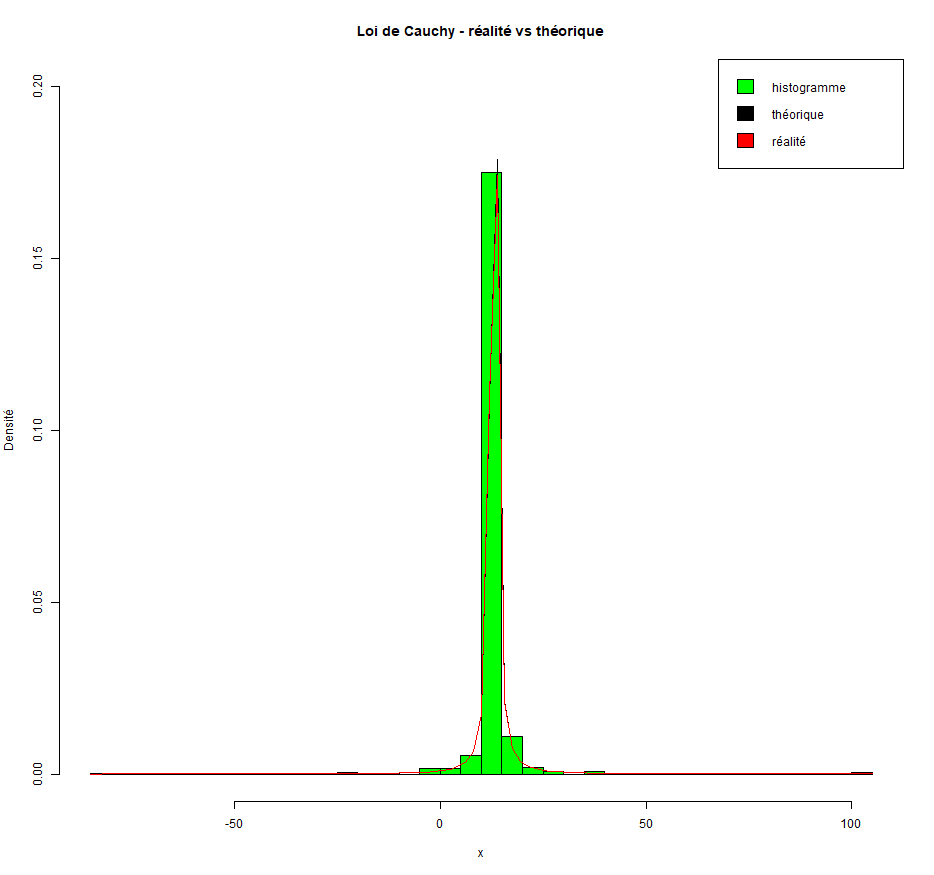
\includegraphics[width=\linewidth]{images/Cauchy_real_vs_theo.png}
\caption{Représentation de l'histogramme et de la courbe de densité}
\end{figure}

Pour $x_0=13$ et $a=0.5$, les valeurs trouvées par R sont $\hat{x_0} = 12.9877139$ et $\hat{a} = 0.4951073$.

\subsection{Test de paramètres}

Nous testons ici si les valeurs trouvées par R sont vraiment approchées à celles théoriques. Pour l'instant, nous n'avons pas d'outils pour vérifier 2 variables en couple.

\subsection{Test d'adéquation}

R nous donne la fonction \emph{ks.test} pour valider la compabilité d'une échantillon avec une loi selon le test de Kolmogorov-Smirnov.

\lstinputlisting[firstline=51, lastline=51]{src/Cauchy.R}

On a trouvé $D = 0.02696$, $p-value = 0.4614$, signifiant l'écart maximale est $0.02696$ et le niveau d'acceptance est $0.4614$. Vu que nous fixons $\alpha = 5\% < p-value$, l'échantillon dépasse largement le test. Autrement dit, il se distribue selon la loi de Cauchy.

\subsection{Etude de biais d'estimateur}

Maintenant on s'intéresse au biais d'estimateur. On relance l'algorithme en-dessus avec de différents observations ($N = 100, 125, 150,..., 1100$). $x_0 = 13$ et $a = 0.5$.

\lstinputlisting{src/Cauchy-variN.R}

\begin{figure}[h]
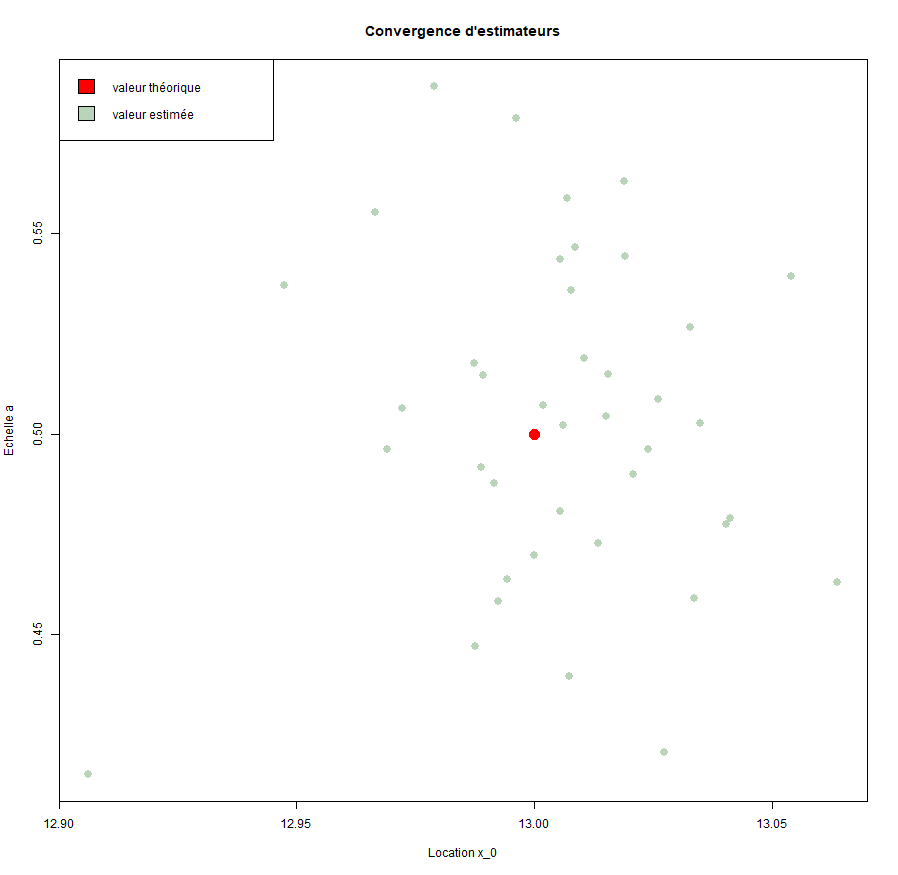
\includegraphics[width=\linewidth]{images/Cauchy_convergence_parametres.png}
\caption{Convergences de $\hat{x_0}$ et $\hat{a}$ vers valeurs théoriques}
\end{figure}

Nous observons que les valeurs estimées se rassemblent assez proches de la valeur théorique.

\subsection{Etude de loi d'extremum}

Générons donc des échantillons de $n$ valeurs ($n=10, 100, 1000, etc.$). Parmi chacun, $\frac{n}{10}$ valeurs les plus grandes seront gardées pour étudier la loi d'extremum.

Comme les réalisations sont indépendantes et identiquement distribuées, théoriquement:
\begin{align*}
{F_{{x_{\max }}}}\left( x \right) & = P\left( {{X_{\max }} \le x} \right)\\
&  = P\left( {{X_1} \le x,...,{X_n} \le x} \right)\\
 & = \prod\limits_{i = 1}^n {{F_X}\left( x \right)} \\
 & = {F_X}{\left( x \right)^n}
\end{align*}

Avec ${F_X}\left( x \right) = \frac{1}{\pi }\arctan \frac{{x - {x_0}}}{a} + \frac{1}{2}$, la fonction de répartition de la loi de Cauchy. Alors, \[{F_{{x_{\max }}}}\left( x \right) = {\left( {\frac{1}{\pi }\arctan \frac{{x - {x_0}}}{a} + \frac{1}{2}} \right)^n}\]

Or, \[\left| {\arctan \frac{{x - {x_0}}}{a}} \right| < \frac{\pi }{2} \Rightarrow \frac{{ - \pi }}{2} < \arctan \frac{{x - {x_0}}}{a} < \frac{\pi }{2} \Rightarrow 0 < \arctan \frac{{x - {x_0}}}{a} + \frac{\pi }{2} < \pi \]

Par conséquence,

\[\begin{array}{l}
\tan \left( {\arctan \frac{{x - {x_0}}}{a} + \frac{\pi }{2}} \right) =  - \cot \left( {\arctan \frac{{x - {x_0}}}{a}} \right) =  - \frac{a}{{x - {x_0}}}\\
 \Rightarrow \arctan \frac{{x - {x_0}}}{a} + \frac{\pi }{2} = \arctan \left( { - \frac{a}{{x - {x_0}}}} \right) = \arctan \frac{a}{{{x_0} - x}}\\
 \Rightarrow {F_{{x_{\max }}}}\left( x \right) = {\pi ^{ - n}}{\left( {\arctan \frac{{x - {x_0}}}{a} + \frac{\pi }{2}} \right)^n} = {\pi ^{ - n}}{\arctan ^n}\frac{a}{{{x_0} - x}}
\end{array}\]
\clearpage

Nous prenons 3 valeurs les plus grandes pour chaque itération, et établissons leur histogramme.
\lstinputlisting[language=R, firstline=1, lastline=39]{src/Cauchy-extreme.R}

\begin{figure}[h]
\centering
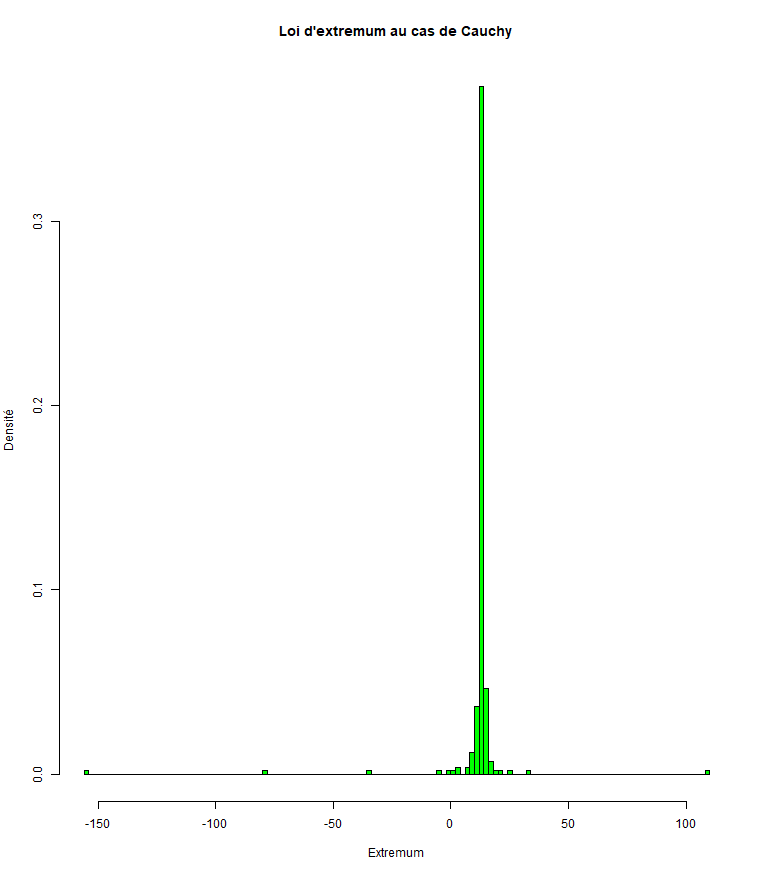
\includegraphics[width=0.8\linewidth]{images/Cauchy_extremum.png}
\caption{Histogramme de valeurs extremum de la distribution de Cauchy}
\end{figure}

En fin d'approximer la loi d'extremum, nous ne regardons que les réalisations positives. En utilisant le package \emph{poweRlaw}, nous calculons la compabilité de la loi d'extremum.

\lstinputlisting[language=R, firstline=41, lastline=50]{src/Cauchy-extreme.R}

\begin{figure}[h]
\centering
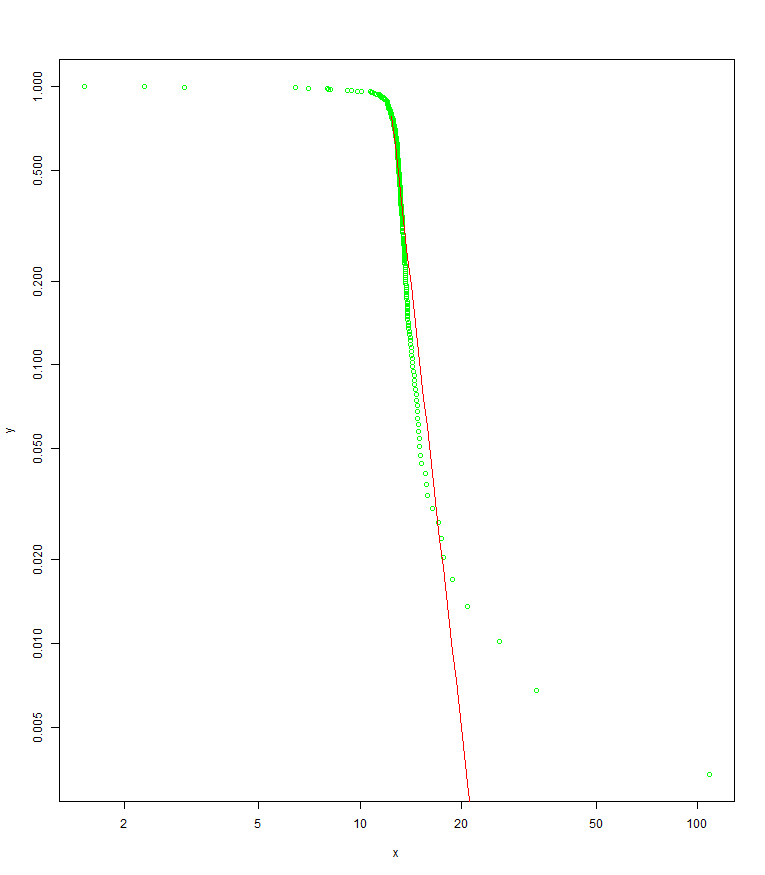
\includegraphics[width=0.8\linewidth]{images/Cauchy_extremum_fitting.png}
\caption{Approcher la loi d'extremum avec celle des maximales de Cauchy. Les données (verte) ne s'approchent pas totalement l'approximation (rouge).}
\end{figure}

Calcul de $p-value$ nous retourne $0$, qui signifie l'incompabilité de ces deux lois.
\clearpage

\section{Loi géométrique}

La loi géomètrique est une loi discrète de distribution utilisé
dans le cadre d'un enchainement (non fini) d'épreuves de Bernouilli. Soit
X une varaible aléatoire suivant cette loi, on a:
\[P(X=k) = (1-p)^(k-1)p\ k\in\mathbb{N}_{+}\]
La variable X est le numéro de la première épreuve où l'on obtient un succès
qui a une probabilité p. Ainsi, p est le seul paramètre de loi (à estimer).
La fonction de répartition $F(k) = P(X\leq{}k)\ k\in\mathbb{N}_{+}$ est:
\[F(k)=1-(1-p)^{k}\]
\begin{proof}
On peut remarquer que:
\[P(X=k)=(1-p)^{k-1}(1-(1-p))=(1-p)^{k-1}-(1-p)^{k}\]
Donc :
\begin{align*}
F(k) & =\sum\limits_{l=1}^{k}P(X=l)=\sum\limits_{l=1}^{k}((1-p)^{l-1}-(1-p)^{l}) \\
F(k) & =\sum\limits_{l=0}^{k-1}(1-p)^{l}-\sum\limits_{l=1}^{k}(1-p)^{l}
\end{align*}
Soit $q=1-p$, on a :
\begin{align*}
F(k) & =\sum\limits_{l=0}^{k-1}q^{l}-\sum\limits_{l=1}^{k}q^{l}\\
F(k) & =\frac{1-p^k}{1-q}-(\frac{1-q^{k+1}}{1-q}-1) \\ 
F(k) & =\frac{1-q^k-1+q^{k+1}+1-q}{1-q} \\
F(k) & =\frac{1-q+q^{k+1}-q^k}{1-q} \\
F(k) & =\frac{1-q-q^k(1-q)}{1-q} \\ 
F(k) & =\frac{1-q-q^k(1-q)}{1-q} \\
F(k) & =1-q^k
\end{align*}

On retrouve bien :
\[F(k)=1-(1-p)^k\]
\end{proof}

\subsection{Génération de n variables aléatoires}

Afin de voir à quoi ressemble la distribution et de pouvoir tester l'estimateur que
nous allons calculer par la suite, on génère des échantillons de 50, 500 et 5000 variables.
On utilise ainsi le code Matlab (Octave) ce dessous :

\lstinputlisting[language=Matlab, firstline=3, lastline=28]{src/geom.m}

On obtient ainsi la figure \ref{Histogrammes et distribution de loi géométrique}.

\begin{figure}[!h]
\label{Histogrammes et distribution de loi géométrique}
\centering
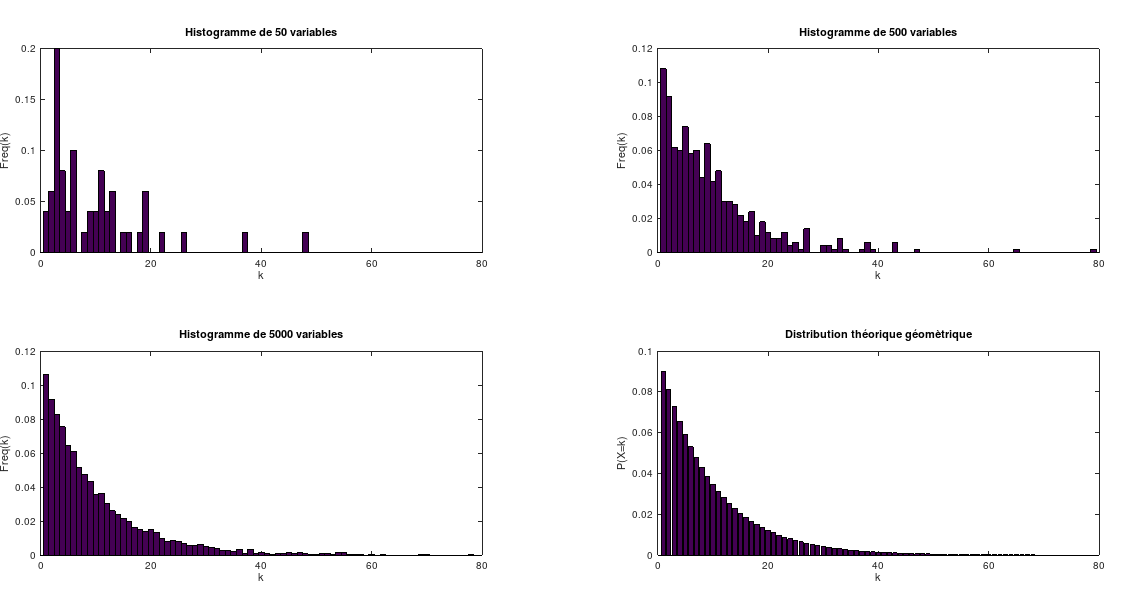
\includegraphics[scale=0.3]{images/histGeom.png} 
\caption{Histogrammes et distribution de loi géométrique}
\end{figure}

Pour générer les populations (voir figure \ref{Histogrammes et distribution de loi géométrique} , on utilise la fonction "geomGen" qui simule $n$ expériences où, pour chacune d'entre elle, on effectue un enchainement
d'épreuve de Bernouilli en générant une variable de loi uniforme sur
$[0;1]$ . Si la valeur obtenu est supérieure à p, on arrête la boucle
et la valeur générée est égale au nombre d'épreuves, sinon on continue 
jusqu'à obtenir cette condition. Le code Matlab (Octave) utilisé est :

\lstinputlisting[language=Matlab]{src/geomGen.m}


\subsection{Estimateurs du maximum de vraisemblance}

L'estimateur $\hat{p}$ du maximum de vraisemblance est la valeur qui
maximise la loi de vraisemblance $L(p)$ : $\hat{p}=argmax(L(p))$.
On calcule $L(p)$ dans un premier temps :
\[L(p)=L(X_1(p),X_2(p),...,X_n(p))=\prod\limits_{i=1}^{n}(1-p)^{X_i-1}p \]
avec $X_i,\ i\in\{1,..,n\}$ les variables d'échantillon.
\[L(p)=p^n(1-p)^{(\sum\limits_{i=1}^{n}X_i)-n}\]
On peut effectuer un passage au logarithme pour trouver un maximum car il s'agit
d'une fonction strictement croissante (et défini sur $]0;1]$). L'argument du maximum du logarithme
de $L(p)$ et du maximum de $L(p)$ sont les mêmes.
\[\log{L(p)}=n\log{p}+(\sum\limits_{i=1}^{n}X_i)-n\]

\begin{thebibliography}{3}
\bibitem{WikiLoiCauchy}

Wikipedia,

\url{https://en.wikipedia.org/wiki/Cauchy_distribution}

\end{thebibliography}
\end{document}